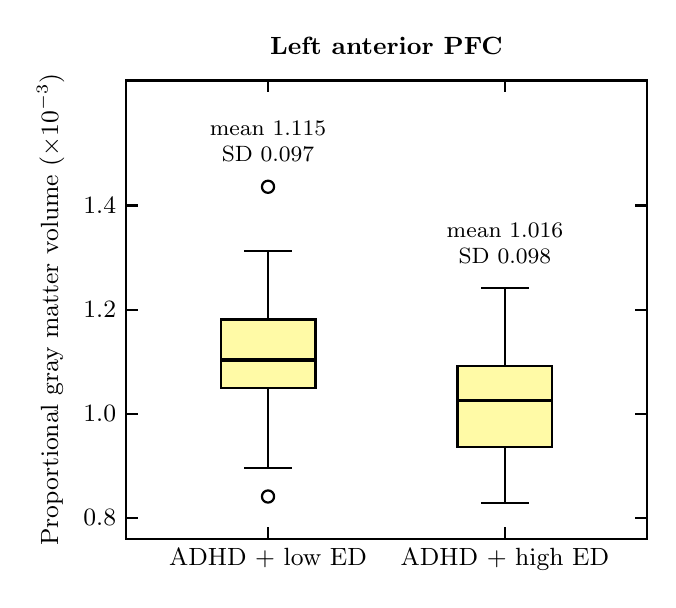
\begin{tikzpicture}[font=\small]
\begin{axis}[
  width=8.2cm, height=7.4cm,
  xmin=0.4, xmax=2.6, ymin=0.76, ymax=1.64,
  xtick={1,2}, xticklabels={ADHD + low ED, ADHD + high ED},
  ytick={0.8,1.0,1.2,1.4},
  yticklabel style={/pgf/number format/fixed, /pgf/number format/precision=1, /pgf/number format/fixed zerofill},
  ylabel={Proportional gray matter volume ($\times 10^{-3}$)},
  title={\textbf{Left anterior PFC}},
  axis line style={thick}, tick style={thick, black},
  clip=false]
% ---------- ADHD + low ED ----------
% whiskers
\draw[thick] (axis cs:1,0.896) -- (axis cs:1,1.050);
\draw[thick] (axis cs:1,1.181) -- (axis cs:1,1.313);
\draw[thick] (axis cs:0.9,0.896) -- (axis cs:1.1,0.896);
\draw[thick] (axis cs:0.9,1.313) -- (axis cs:1.1,1.313);
% box and median
\filldraw[thick, fill=yellow!35] (axis cs:0.8,1.050) rectangle (axis cs:1.2,1.181);
\draw[very thick] (axis cs:0.8,1.103) -- (axis cs:1.2,1.103);
% outliers
\draw[thick] (axis cs:1,1.436) circle (2.2pt);
\draw[thick] (axis cs:1,0.841) circle (2.2pt);
% mean and SD
\node[align=center, anchor=south, font=\footnotesize] at (axis cs:1,1.465) {mean $1.115$\\SD $0.097$};
% ---------- ADHD + high ED ----------
\draw[thick] (axis cs:2,0.828) -- (axis cs:2,0.936);
\draw[thick] (axis cs:2,1.091) -- (axis cs:2,1.242);
\draw[thick] (axis cs:1.9,0.828) -- (axis cs:2.1,0.828);
\draw[thick] (axis cs:1.9,1.242) -- (axis cs:2.1,1.242);
\filldraw[thick, fill=yellow!35] (axis cs:1.8,0.936) rectangle (axis cs:2.2,1.091);
\draw[very thick] (axis cs:1.8,1.025) -- (axis cs:2.2,1.025);
\node[align=center, anchor=south, font=\footnotesize] at (axis cs:2,1.27) {mean $1.016$\\SD $0.098$};
\end{axis}
\end{tikzpicture}
